\section{Motivación}

Desde hace ya unos años, estamos viviendo una revolución en el desarrollo web, que a provocado un cambio en nuestro estilo de vida, la forma de comunicarnos, en los flujos de información e incluso en nuestras relaciones diarias. HTML\footnote{Hypertext Markup Language} y JavaScript son una parte importante de esta revolución, y es por ello, que decidí dar el paso y crear una aplicación que funcionará única y exclusivamente en el navegador (sin necesidad de un servidor). 

Estamos viendo como día a día, aplicaciones que han sido por antonomasia nativas (editores de texto, hojas de cálculo, aplicaciones de gestión, juegos ...), están siendo implementadas con tecnologías web con gran éxito. Los editores de mapas mentales también han dado ese paso existen aplicaciones como text2mindmap\footnote{http://www.text2mindmap.com/}, MindMeister\footnote{http://www.mindmeister.com/es}, etc., tan versátiles o más que las propias aplicaciones nativas.

Hace ya tiempo que vio la luz los primeros borradores de HTML5\footnote{El primer borrador de HTML5 fue publicado en 2008} (ver figura \ref{fig:html5}) pero su implantación está siendo lenta, no sólo por parte de la comunidad de desarrolladores y diseñadores, sino también por parte de los navegadores. 

HTML5 ha tomado en cuenta los defectos de su versión anterior\footnote{HTML 4.01} y mejorar otras características como: 

\begin{figure}[htbp]
\centering
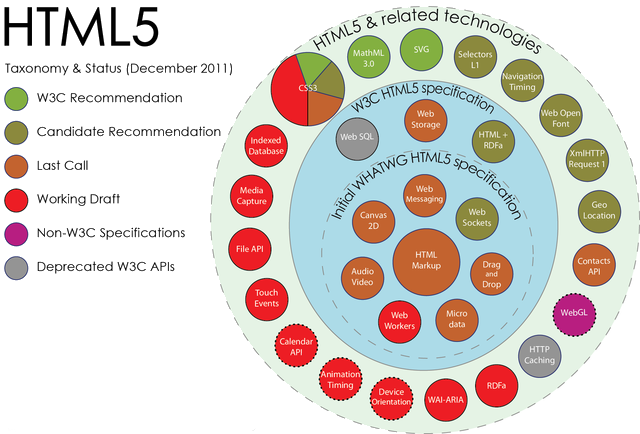
\includegraphics[width=1.1\textwidth]{imagenes/html5}
\caption{Esquema general de la especificación HTML5 a diciembre de 2011}
\label{fig:html5}
\end{figure}


\begin{itemize}
\item \textbf{Nuevas etiquetas estructurales.} Se ha incorporado un nuevo conjunto de etiquetas pensadas para definir mejor la estructura de una web, entre las más importantes están las de encabezado, barra de navegación, secciones y pie.

\item \textbf{Manejo de imágenes.} En la versión anterior podía incorporar imágenes ahora, además podemos modificarlas e interactuar con ellas. También disponemos un una etiqueta y un API completo para manejo de canvas\footnote{En principio, sólo en 2D.}.

\item \textbf{Etiquetas de vídeo y audio.} Sin incluir flash ni aplicaciones externas podemos incorporar un reproductor de vídeo y/o audio. 

\item \textbf{Mejora en la semántica web.} HTML5 incluye elementos que permiten dar información de la página web a los buscadores para obtener resultados adaptados a las necesidades del usuario.

\item \textbf{Soporte móvil/tabletas.} Mejoras en las hojas de estilos, nuevos manejadores para evento touch, etc.

\item \textbf{Acceso a ficheros.} Incorpora un API para lectura/escritura de ficheros.
  
\end{itemize}

La motivación no puede ser otra que profundizar en las características de HTML5 y aprender de esta tecnología. 
